%%%%%%%%%%%%%%%%%%%%%%%%%%%%%%%%%%%%%%%%%%%%%%%%%%%%%%%%%%%%%%%
%
% Welcome to Overleaf --- just edit your LaTeX on the left,
% and we'll compile it for you on the right. If you open the
% 'Share' menu, you can invite other users to edit at the same
% time. See www.overleaf.com/learn for more info. Enjoy!
%
%%%%%%%%%%%%%%%%%%%%%%%%%%%%%%%%%%%%%%%%%%%%%%%%%%%%%%%%%%%%%%%


% Inbuilt themes in beamer
\documentclass{beamer}

% Theme choice:
\usetheme{CambridgeUS}

% Title page details: 
\title{Assignment 9} 
\author{Donal Loitam - AI21BTECH11009}
\date{\today}
\logo{\large \LaTeX{}}

\usepackage{hyperref}
\usepackage{mathtools}
\usepackage{amssymb}
\usepackage{amsmath}


\begin{document}

% Title page frame
\begin{frame}
    \titlepage 
\end{frame}

% Remove logo from the next slides
\logo{}


% Outline frame
\begin{frame}{Papoulis chap 5 Ex 5.2}
TABLE OF CONTENTS
    \tableofcontents
\end{frame}


% Lists frame
\section{Question}
\begin{frame}{Problem}
Q)The distribution of $ax+b$. 
\end{frame}

\section{Solution}
\begin{frame}{Solution}
    Let $y = ax+b$ \\
    To find $F_y(y)$, we must find the values of $x$ such that $ax+b \le y$.
    \begin{itemize}
        \item a) if $a > 0$, then $ax+b \le y$ for $x \le \frac{y-b}{a}$. Hence 
        \begin{align}
            F_y(y) = P(x \le \frac{y-b}{a})= F_x(\frac{y-b}{a}) , \hspace{5mm}  a>0
        \end{align} 

        \item b) if $a < 0$, then $ax+b \le y$ for $x > \frac{y-b}{a}$. Hence 
        \begin{align}
            F_y(y) = P(x \ge \frac{y-b}{a})= 1-F_x(\frac{y-b}{a}) , \hspace{5mm}  a<0
        \end{align} 
        

        
    \end{itemize}

\end{frame}

\section{Graph}
\begin{frame}{...}
    \begin{figure}[!ht]
		\centering
		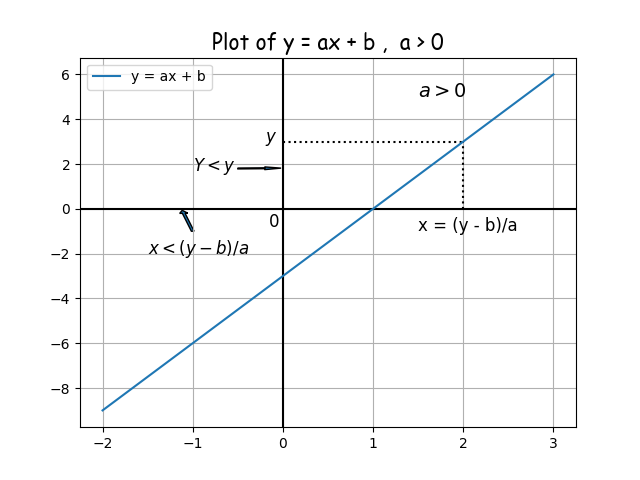
\includegraphics[width=\textwidth,height=6.5cm,keepaspectratio]{line_with_axis.png}
		\caption{FIG 1}
		\label{fig1}
	\end{figure}
\end{frame}

% % Blocks frame
\section{Codes}
\begin{frame}{CODES}
    \begin{block}{Python}
         Download python code from - \href{...}{Python}
    \end{block}

 \begin{block}{Beamer}
         Download Beamer code from - \href{...}{Beamer}
    \end{block}
\end{frame} 

\end{document}
